%\documentclass[pra,showpacs,showkeys,amsfonts,amsmath,twocolumn]{revtex4}
\documentclass[amsmath,blue,handout]{beamer}
%\documentclass[pra,showpacs,showkeys,amsfonts]{revtex4}
\usepackage[T1]{fontenc}
\usepackage{beamerthemeshadow}
%\usepackage[dark]{beamerthemesidebar}
%\usepackage[headheight=24pt,footheight=12pt]{beamerthemesplit}
%\usepackage{beamerthemesplit}
%\usepackage[bar]{beamerthemetree}
\usepackage{graphicx}
\usepackage{pgf}

%\RequirePackage[german]{babel}
%\selectlanguage{german}
%\RequirePackage[isolatin]{inputenc}

\pgfdeclareimage[height=0.5cm]{logo}{tu-logo}
\logo{\pgfuseimage{logo}}
\beamertemplatetriangleitem
\begin{document}

\title{\bf Quantum correlations \& beyond}
%\subtitle{Naturwissenschaftlich-Humanisticher Tag am BG 19\\Weltbild und Wissenschaft\\http://tph.tuwien.ac.at/\~{}svozil/publ/2005-BG18-pres.pdf}
\subtitle{http://tph.tuwien.ac.at/$\sim$svozil/publ/2005-gdansk-pres.pdf}
\author{Karl Svozil}
\institute{Institut f\"ur Theoretische Physik, University of Technology Vienna, \\
Wiedner Hauptstra\ss e 8-10/136, A-1040 Vienna, Austria\\
svozil@tuwien.ac.at
%{\tiny Disclaimer: Die hier vertretenen Meinungen des Autors verstehen sich als Diskussionsbeitr�ge und decken sich nicht notwendigerweise mit den Positionen der Technischen Universit�t Wien oder deren Vertreter.}
}
\date{Oct. 19, 2005}
\maketitle

\frame{\tableofcontents}



\section{Classical, quantum \& stronger-than-quantum correlations}
\subsection{General setup}
\frame{
\frametitle{General setup}



There are two measurement directions ${ a}$ and ${ b}$
of two
dichotomic observables with values ``-1'' and ``1''
at two spatially separated locations.
The measurement direction ${a}$ at ``Alice's location''
is unknown to an observer ``Bob'' measuring ${ b}$ and {\it vice versa}.
A two-particle correlation function $E(\theta )$
with $\theta =\vert {a} - { b}\vert $
is defined by averaging the product of the outcomes $O({ a})_i, O({ b} )_i\in {-1,1}$
in the $i$th experiment; i.e.,  $E(\theta )=(1/N)\sum_{i=1}^N O({ a})_i O({ b})_i$.

}

\subsection{Classical correlations}
\frame{
\frametitle{Classical correlations for two-particle singlet state}

$$E(a,b) = {A_+(a,b)-A_-(a,b)\over 2\pi}= {2A_+(a,b) -2\pi \over 2\pi}={2\over \pi}\vert a-b\vert - 1={2\over \pi}\theta - 1$$

%TeXCAD Picture [1.pic]. Options:
%\grade{\on}
%\emlines{\off}
%\epic{\off}
%\beziermacro{\on}
%\reduce{\on}
%\snapping{\off}
%\quality{8.00}
%\graddiff{0.01}
%\snapasp{1}
%\zoom{4.0000}
\unitlength 0.5mm % = 2.85pt
\linethickness{0.4pt}
\ifx\plotpoint\undefined\newsavebox{\plotpoint}\fi % GNUPLOT compatibility
\begin{picture}(63.52,273.5)(0,0)
%\circle(32.75,234.75){61.53}
\put(63.52,234.75){\line(0,1){1.227}}
\put(63.49,235.98){\line(0,1){1.225}}
\multiput(63.42,237.2)(-.0305,.3052){4}{\line(0,1){.3052}}
\multiput(63.3,238.42)(-.02846,.20252){6}{\line(0,1){.20252}}
\multiput(63.13,239.64)(-.03129,.17247){7}{\line(0,1){.17247}}
\multiput(62.91,240.84)(-.03338,.1497){8}{\line(0,1){.1497}}
\multiput(62.64,242.04)(-.03146,.1186){10}{\line(0,1){.1186}}
\multiput(62.32,243.23)(-.03287,.10659){11}{\line(0,1){.10659}}
\multiput(61.96,244.4)(-.03139,.089015){13}{\line(0,1){.089015}}
\multiput(61.56,245.56)(-.03242,.081428){14}{\line(0,1){.081428}}
\multiput(61.1,246.7)(-.033265,.074733){15}{\line(0,1){.074733}}
\multiput(60.6,247.82)(-.031958,.064718){17}{\line(0,1){.064718}}
\multiput(60.06,248.92)(-.032596,.05987){18}{\line(0,1){.05987}}
\multiput(59.47,250)(-.033117,.055443){19}{\line(0,1){.055443}}
\multiput(58.84,251.05)(-.033537,.051374){20}{\line(0,1){.051374}}
\multiput(58.17,252.08)(-.032326,.045451){22}{\line(0,1){.045451}}
\multiput(57.46,253.08)(-.032629,.042207){23}{\line(0,1){.042207}}
\multiput(56.71,254.05)(-.032858,.03917){24}{\line(0,1){.03917}}
\multiput(55.92,254.99)(-.033018,.036315){25}{\line(0,1){.036315}}
\multiput(55.1,255.9)(-.033115,.033625){26}{\line(0,1){.033625}}
\multiput(54.24,256.77)(-.035807,.033569){25}{\line(-1,0){.035807}}
\multiput(53.34,257.61)(-.038663,.033452){24}{\line(-1,0){.038663}}
\multiput(52.41,258.41)(-.041704,.03327){23}{\line(-1,0){.041704}}
\multiput(51.45,259.18)(-.044952,.033017){22}{\line(-1,0){.044952}}
\multiput(50.46,259.9)(-.048434,.032683){21}{\line(-1,0){.048434}}
\multiput(49.45,260.59)(-.052184,.032262){20}{\line(-1,0){.052184}}
\multiput(48.4,261.24)(-.059365,.033507){18}{\line(-1,0){.059365}}
\multiput(47.34,261.84)(-.064222,.032943){17}{\line(-1,0){.064222}}
\multiput(46.24,262.4)(-.069577,.032253){16}{\line(-1,0){.069577}}
\multiput(45.13,262.92)(-.080923,.033661){14}{\line(-1,0){.080923}}
\multiput(44,263.39)(-.088524,.032746){13}{\line(-1,0){.088524}}
\multiput(42.85,263.81)(-.09724,.03162){12}{\line(-1,0){.09724}}
\multiput(41.68,264.19)(-.11811,.03326){10}{\line(-1,0){.11811}}
\multiput(40.5,264.52)(-.1326,.0317){9}{\line(-1,0){.1326}}
\multiput(39.31,264.81)(-.15048,.02968){8}{\line(-1,0){.15048}}
\multiput(38.1,265.05)(-.20206,.03155){6}{\line(-1,0){.20206}}
\multiput(36.89,265.24)(-.24379,.02816){5}{\line(-1,0){.24379}}
\put(35.67,265.38){\line(-1,0){1.224}}
\put(34.45,265.47){\line(-1,0){1.226}}
\put(33.22,265.51){\line(-1,0){1.227}}
\put(31.99,265.51){\line(-1,0){1.226}}
\put(30.77,265.45){\line(-1,0){1.223}}
\multiput(29.54,265.35)(-.24351,-.03043){5}{\line(-1,0){.24351}}
\multiput(28.33,265.2)(-.20175,-.03343){6}{\line(-1,0){.20175}}
\multiput(27.12,265)(-.1502,-.03109){8}{\line(-1,0){.1502}}
\multiput(25.91,264.75)(-.1323,-.03293){9}{\line(-1,0){.1323}}
\multiput(24.72,264.45)(-.10708,-.03124){11}{\line(-1,0){.10708}}
\multiput(23.55,264.11)(-.09694,-.03253){12}{\line(-1,0){.09694}}
\multiput(22.38,263.72)(-.088215,-.03357){13}{\line(-1,0){.088215}}
\multiput(21.24,263.28)(-.075232,-.03212){15}{\line(-1,0){.075232}}
\multiput(20.11,262.8)(-.069274,-.032901){16}{\line(-1,0){.069274}}
\multiput(19,262.27)(-.063912,-.03354){17}{\line(-1,0){.063912}}
\multiput(17.91,261.7)(-.055942,-.032266){19}{\line(-1,0){.055942}}
\multiput(16.85,261.09)(-.051881,-.032748){20}{\line(-1,0){.051881}}
\multiput(15.81,260.43)(-.048127,-.033134){21}{\line(-1,0){.048127}}
\multiput(14.8,259.74)(-.044642,-.033434){22}{\line(-1,0){.044642}}
\multiput(13.82,259)(-.041392,-.033658){23}{\line(-1,0){.041392}}
\multiput(12.87,258.23)(-.036816,-.032459){25}{\line(-1,0){.036816}}
\multiput(11.95,257.42)(-.034127,-.032597){26}{\line(-1,0){.034127}}
\multiput(11.06,256.57)(-.0328,-.033932){26}{\line(0,-1){.033932}}
\multiput(10.21,255.69)(-.032678,-.036622){25}{\line(0,-1){.036622}}
\multiput(9.39,254.77)(-.032491,-.039474){24}{\line(0,-1){.039474}}
\multiput(8.61,253.82)(-.0337,-.044442){22}{\line(0,-1){.044442}}
\multiput(7.87,252.85)(-.03342,-.047929){21}{\line(0,-1){.047929}}
\multiput(7.17,251.84)(-.033056,-.051685){20}{\line(0,-1){.051685}}
\multiput(6.51,250.81)(-.032599,-.055749){19}{\line(0,-1){.055749}}
\multiput(5.89,249.75)(-.032036,-.060172){18}{\line(0,-1){.060172}}
\multiput(5.31,248.66)(-.033313,-.069076){16}{\line(0,-1){.069076}}
\multiput(4.78,247.56)(-.032567,-.07504){15}{\line(0,-1){.07504}}
\multiput(4.29,246.43)(-.03166,-.081727){14}{\line(0,-1){.081727}}
\multiput(3.85,245.29)(-.03311,-.09675){12}{\line(0,-1){.09675}}
\multiput(3.45,244.13)(-.03188,-.1069){11}{\line(0,-1){.1069}}
\multiput(3.1,242.95)(-.03372,-.1321){9}{\line(0,-1){.1321}}
\multiput(2.79,241.76)(-.03198,-.15001){8}{\line(0,-1){.15001}}
\multiput(2.54,240.56)(-.02968,-.17276){7}{\line(0,-1){.17276}}
\multiput(2.33,239.35)(-.03188,-.24333){5}{\line(0,-1){.24333}}
\put(2.17,238.14){\line(0,-1){1.222}}
\put(2.06,236.92){\line(0,-1){1.225}}
\put(2,235.69){\line(0,-1){1.227}}
\put(1.99,234.46){\line(0,-1){1.227}}
\put(2.02,233.24){\line(0,-1){1.224}}
\multiput(2.11,232.01)(.0334,-.3049){4}{\line(0,-1){.3049}}
\multiput(2.24,230.79)(.03034,-.20224){6}{\line(0,-1){.20224}}
\multiput(2.42,229.58)(.0329,-.17218){7}{\line(0,-1){.17218}}
\multiput(2.65,228.37)(.03091,-.13279){9}{\line(0,-1){.13279}}
\multiput(2.93,227.18)(.03256,-.1183){10}{\line(0,-1){.1183}}
\multiput(3.26,226)(.03104,-.09743){12}{\line(0,-1){.09743}}
\multiput(3.63,224.83)(.032218,-.088718){13}{\line(0,-1){.088718}}
\multiput(4.05,223.67)(.033178,-.081123){14}{\line(0,-1){.081123}}
\multiput(4.51,222.54)(.031838,-.069768){16}{\line(0,-1){.069768}}
\multiput(5.02,221.42)(.03256,-.064417){17}{\line(0,-1){.064417}}
\multiput(5.57,220.33)(.033152,-.059564){18}{\line(0,-1){.059564}}
\multiput(6.17,219.25)(.033633,-.055132){19}{\line(0,-1){.055132}}
\multiput(6.81,218.21)(.032394,-.048628){21}{\line(0,-1){.048628}}
\multiput(7.49,217.19)(.032748,-.045148){22}{\line(0,-1){.045148}}
\multiput(8.21,216.19)(.033021,-.041901){23}{\line(0,-1){.041901}}
\multiput(8.97,215.23)(.033221,-.038862){24}{\line(0,-1){.038862}}
\multiput(9.77,214.3)(.033355,-.036006){25}{\line(0,-1){.036006}}
\multiput(10.6,213.4)(.033427,-.033315){26}{\line(1,0){.033427}}
\multiput(11.47,212.53)(.036118,-.033233){25}{\line(1,0){.036118}}
\multiput(12.37,211.7)(.038973,-.03309){24}{\line(1,0){.038973}}
\multiput(13.31,210.9)(.042012,-.03288){23}{\line(1,0){.042012}}
\multiput(14.28,210.15)(.045258,-.032596){22}{\line(1,0){.045258}}
\multiput(15.27,209.43)(.048737,-.03223){21}{\line(1,0){.048737}}
\multiput(16.29,208.75)(.055245,-.033447){19}{\line(1,0){.055245}}
\multiput(17.34,208.12)(.059675,-.032952){18}{\line(1,0){.059675}}
\multiput(18.42,207.53)(.064526,-.032343){17}{\line(1,0){.064526}}
\multiput(19.51,206.98)(.074533,-.03371){15}{\line(1,0){.074533}}
\multiput(20.63,206.47)(.081234,-.032905){14}{\line(1,0){.081234}}
\multiput(21.77,206.01)(.088826,-.03192){13}{\line(1,0){.088826}}
\multiput(22.92,205.59)(.1064,-.03351){11}{\line(1,0){.1064}}
\multiput(24.1,205.23)(.11841,-.03216){10}{\line(1,0){.11841}}
\multiput(25.28,204.9)(.13289,-.03046){9}{\line(1,0){.13289}}
\multiput(26.48,204.63)(.17228,-.03232){7}{\line(1,0){.17228}}
\multiput(27.68,204.4)(.20234,-.02966){6}{\line(1,0){.20234}}
\multiput(28.9,204.23)(.305,-.0324){4}{\line(1,0){.305}}
\put(30.12,204.1){\line(1,0){1.224}}
\put(31.34,204.02){\line(1,0){1.227}}
\put(32.57,203.98){\line(1,0){1.227}}
\put(33.79,204){\line(1,0){1.225}}
\put(35.02,204.07){\line(1,0){1.222}}
\multiput(36.24,204.18)(.24322,.0327){5}{\line(1,0){.24322}}
\multiput(37.46,204.35)(.17266,.03026){7}{\line(1,0){.17266}}
\multiput(38.67,204.56)(.1499,.03248){8}{\line(1,0){.1499}}
\multiput(39.86,204.82)(.11879,.03075){10}{\line(1,0){.11879}}
\multiput(41.05,205.13)(.10679,.03224){11}{\line(1,0){.10679}}
\multiput(42.23,205.48)(.09663,.03343){12}{\line(1,0){.09663}}
\multiput(43.39,205.88)(.08162,.031935){14}{\line(1,0){.08162}}
\multiput(44.53,206.33)(.07493,.03282){15}{\line(1,0){.07493}}
\multiput(45.65,206.82)(.068964,.033545){16}{\line(1,0){.068964}}
\multiput(46.76,207.36)(.060063,.032238){18}{\line(1,0){.060063}}
\multiput(47.84,207.94)(.055639,.032786){19}{\line(1,0){.055639}}
\multiput(48.89,208.56)(.051573,.03323){20}{\line(1,0){.051573}}
\multiput(49.93,209.22)(.047816,.033581){21}{\line(1,0){.047816}}
\multiput(50.93,209.93)(.042401,.032377){23}{\line(1,0){.042401}}
\multiput(51.91,210.67)(.039365,.032624){24}{\line(1,0){.039365}}
\multiput(52.85,211.46)(.036511,.032801){25}{\line(1,0){.036511}}
\multiput(53.76,212.28)(.033822,.032914){26}{\line(1,0){.033822}}
\multiput(54.64,213.13)(.032482,.034236){26}{\line(0,1){.034236}}
\multiput(55.49,214.02)(.033682,.038463){24}{\line(0,1){.038463}}
\multiput(56.3,214.95)(.033518,.041505){23}{\line(0,1){.041505}}
\multiput(57.07,215.9)(.033284,.044754){22}{\line(0,1){.044754}}
\multiput(57.8,216.89)(.032971,.048239){21}{\line(0,1){.048239}}
\multiput(58.49,217.9)(.032573,.051991){20}{\line(0,1){.051991}}
\multiput(59.14,218.94)(.032078,.056051){19}{\line(0,1){.056051}}
\multiput(59.75,220)(.033325,.064025){17}{\line(0,1){.064025}}
\multiput(60.32,221.09)(.032667,.069384){16}{\line(0,1){.069384}}
\multiput(60.84,222.2)(.031866,.07534){15}{\line(0,1){.07534}}
\multiput(61.32,223.33)(.033273,.088328){13}{\line(0,1){.088328}}
\multiput(61.75,224.48)(.0322,.09705){12}{\line(0,1){.09705}}
\multiput(62.14,225.65)(.03088,.10719){11}{\line(0,1){.10719}}
\multiput(62.48,226.82)(.03249,.13241){9}{\line(0,1){.13241}}
\multiput(62.77,228.02)(.03058,.1503){8}{\line(0,1){.1503}}
\multiput(63.01,229.22)(.03275,.20187){6}{\line(0,1){.20187}}
\multiput(63.21,230.43)(.02961,.24361){5}{\line(0,1){.24361}}
\put(63.36,231.65){\line(0,1){1.223}}
\put(63.46,232.87){\line(0,1){1.879}}
%\end
\put(32.75,235.25){\line(0,1){30.5}}
%\dottedline(1.75,235.75)(2,235.25)
\multiput(1.68,235.68)(.125,-.25){3}{{\rule{.4pt}{.4pt}}}
%\end
%\dottedline(2,235.25)(63.5,234.75)
\multiput(1.93,235.18)(.99194,-.00806){63}{{\rule{.4pt}{.4pt}}}
%\end
%\dottedline(9.5,255.5)(55.75,214.25)
\multiput(9.43,255.43)(.72266,-.64453){65}{{\rule{.4pt}{.4pt}}}
%\end
%\emline(32.75,235)(54.75,256.5)
\multiput(32.75,235)(.034482759,.03369906){638}{\line(1,0){.034482759}}
%\end
\put(32.75,273.5){\makebox(0,0)[cc]{$a$}}
\put(62,263.5){\makebox(0,0)[cc]{$b$}}
\put(26,218.5){\makebox(0,0)[cc]{$-$}}
\put(53.25,245.5){\makebox(0,0)[cc]{$-$}}
\put(8.25,243){\makebox(0,0)[cc]{$+$}}
\put(54.75,226.25){\makebox(0,0)[cc]{$+$}}
\end{picture}



 }


\subsection{Quantum correlations}
\frame[shrink=2]{
\frametitle{Quantum correlations for two-particle singlet state}

$$E (\theta ) = {3/[j(j+1)]} C(\theta )$$
with non-normalized
\begin{eqnarray}
C(\theta )&=&
\langle J= 0 ,M= 0\mid \alpha \cdot \hat{J}^A \otimes \beta \cdot
\hat{J}^B\mid
J=0,M=0\rangle
\nonumber
 \\
&=&
 \sum_{m,m'}
\langle  00 \mid jm,j-m \rangle
\langle  jm',j-m'\mid 00 \rangle \times \nonumber
\\
&&
\qquad
\qquad
\qquad
\times
^A\langle jm\mid  ^B\langle j-m\mid
\alpha \cdot \hat{J}^A \otimes \beta \cdot \hat{J}^B
\mid jm'\rangle ^A \mid j-m'\rangle ^B  \nonumber
\\
&=&
 \sum_{m,m'}
\langle  00 \mid jm,j-m \rangle
\langle  jm',j-m'\mid 00 \rangle       \times \nonumber  \\
&&
\qquad
\qquad
\qquad   \times
\langle jm\mid
\alpha \cdot \hat{J}^{A}
\mid jm'\rangle
 \langle j-m\mid
 \beta \cdot \hat{J}^B
 \mid j-m'\rangle                             \nonumber
\\
&=&
 \sum_{m,m'}
{(-1)^{j-m}(-1)^{j-m'}\over 2j+1}
\langle jm\mid
 \hat{J}^A_z
\mid jm'\rangle
\langle j-m\mid
 \beta \cdot \hat{J}^B
 \mid j-m'\rangle \nonumber
\\
&=&
 \sum_{m,m'}
{(-1)^{j-m}(-1)^{j-m'}\over 2j+1}
m \delta _{m m'}
\langle j-m\mid
 \beta \cdot \hat{J}^B
 \mid j-m'\rangle \nonumber
\\
&=&  \sum_m
m{(-1)^{2j-2m}\over 2j+1}
 \langle j-m\mid
 \beta \cdot \hat{J}^B
 \mid j-m\rangle  = {1\over 2j+1}  \sum_m
-m^2 \beta_z      = -{1 \over 2j+1}\cos \theta  \sum_{m=-j}^j
m^2
\qquad {\rm for} \; 0\le \theta \le \pi
 \nonumber
\\
&=&- {j(j+1)\over 3} \, \cos \theta
\qquad {\rm for} \; 0\le \theta \le \pi
\quad .
 \nonumber
\end{eqnarray}

}



\subsection{Stronger-than-quantum correlations}
\frame[shrink=2]{
\frametitle{Stronger-than-quantum correlations}
\begin{itemize}
\item<+->
S. Popescu and D. Rohrlich. Quantum nonlocality as an axiom. Foundations
of Physics, 24(3):379�358, 1994. 
No violation of relativistic causality.

\item<+->
G. Krenn and K. Svozil, ``Stronger-than-quantum correlations'', Foundation of Physics 28(6), 971-984 (1998) [CrossRef DOI:10.1023/A:1018821314465]
 
{\footnotesize
\begin {tabular}{|c|c|c|c|}
\hline\hline
& c & qm & s \\
\hline
\hline
$P^=(\theta ) =2P^{++}(\theta )=2P^{--} (\theta )$&  $\theta /
\pi$ &$\sin^2(\theta /
2)$&$H(2\theta / \pi -1)$\\
$P^{\neq} (\theta )=2P^{+-}(\theta )=2P^{-+} (\theta )$&   $1-\theta /
\pi$ &$\cos^2(\theta /
2)$&$H(1-2\theta / \pi)$\\
\hline
\hline
$E(\theta ) = P^=(\theta ) -P^{\neq} (\theta )  $& $2\theta / \pi -1$
&$-\cos({\theta })$&${\mbox sgn}(2\theta / \pi -1 )$\\
\hline
\hline
\end {tabular}
}
\end{itemize} 
        }



\frame[shrink=2]{
\frametitle{Stronger-than-quantum correlations cntd.}
\begin{center}
%TexCad Options
%\grade{\off}
%\emlines{\off}
%\beziermacro{\off}
%\reduce{\on}
%\snapping{\off}
%\quality{4.00}
%\graddiff{0.01}
%\snapasp{1}
%\zoom{1.00}
\unitlength 1.00mm
\linethickness{0.4pt}
\begin{picture}(102.00,102.00)
%\emline(10.00,10.00)(10.00,100.00)
\put(10.00,10.00){\line(0,1){90.00}}
%\end
\put(10.00,55.00){\line(1,0){45.00}}
\put(55.00,55.00){\line(1,0){45.00}}
\put(10.00,10.00){\line(1,1){90.00}}
\put(100.00,100.00){\line(-1,0){45.00}}
\put(10.00,10.00){\line(1,0){45.00}}
%\bezier{284}(10.00,10.00)(30.00,10.00)(55.00,55.00)
\put(10.00,10.00){\line(1,0){1.41}}
\multiput(11.41,10.06)(0.71,0.08){2}{\line(1,0){0.71}}
\multiput(12.84,10.22)(0.48,0.09){3}{\line(1,0){0.48}}
\multiput(14.28,10.50)(0.36,0.10){4}{\line(1,0){0.36}}
\multiput(15.73,10.89)(0.29,0.10){5}{\line(1,0){0.29}}
\multiput(17.20,11.39)(0.25,0.10){6}{\line(1,0){0.25}}
\multiput(18.67,12.01)(0.21,0.10){7}{\line(1,0){0.21}}
\multiput(20.16,12.73)(0.21,0.12){7}{\line(1,0){0.21}}
\multiput(21.66,13.57)(0.19,0.12){8}{\line(1,0){0.19}}
\multiput(23.18,14.52)(0.17,0.12){9}{\line(1,0){0.17}}
\multiput(24.70,15.58)(0.15,0.12){10}{\line(1,0){0.15}}
\multiput(26.24,16.75)(0.14,0.12){11}{\line(1,0){0.14}}
\multiput(27.79,18.03)(0.13,0.12){12}{\line(1,0){0.13}}
\multiput(29.36,19.43)(0.12,0.12){13}{\line(1,0){0.12}}
\multiput(30.93,20.94)(0.11,0.12){14}{\line(0,1){0.12}}
\multiput(32.52,22.55)(0.11,0.12){14}{\line(0,1){0.12}}
\multiput(34.12,24.28)(0.12,0.13){14}{\line(0,1){0.13}}
\multiput(35.74,26.12)(0.12,0.14){14}{\line(0,1){0.14}}
\multiput(37.36,28.08)(0.12,0.15){14}{\line(0,1){0.15}}
\multiput(39.00,30.14)(0.12,0.16){14}{\line(0,1){0.16}}
\multiput(40.65,32.32)(0.12,0.16){14}{\line(0,1){0.16}}
\multiput(42.31,34.60)(0.12,0.17){14}{\line(0,1){0.17}}
\multiput(43.99,37.00)(0.11,0.17){15}{\line(0,1){0.17}}
\multiput(45.67,39.51)(0.11,0.17){15}{\line(0,1){0.17}}
\multiput(47.37,42.14)(0.11,0.18){15}{\line(0,1){0.18}}
\multiput(49.09,44.87)(0.11,0.19){15}{\line(0,1){0.19}}
\multiput(50.81,47.72)(0.12,0.20){15}{\line(0,1){0.20}}
\multiput(52.55,50.67)(0.12,0.21){21}{\line(0,1){0.21}}
%\end
%\bezier{284}(55.00,55.00)(80.00,100.00)(100.00,100.00)
\multiput(55.00,55.00)(0.12,0.21){15}{\line(0,1){0.21}}
\multiput(56.75,58.11)(0.12,0.20){15}{\line(0,1){0.20}}
\multiput(58.50,61.11)(0.12,0.19){15}{\line(0,1){0.19}}
\multiput(60.23,64.00)(0.11,0.19){15}{\line(0,1){0.19}}
\multiput(61.94,66.78)(0.11,0.18){15}{\line(0,1){0.18}}
\multiput(63.65,69.45)(0.11,0.17){15}{\line(0,1){0.17}}
\multiput(65.34,72.01)(0.12,0.17){14}{\line(0,1){0.17}}
\multiput(67.02,74.45)(0.12,0.17){14}{\line(0,1){0.17}}
\multiput(68.69,76.78)(0.12,0.16){14}{\line(0,1){0.16}}
\multiput(70.34,79.00)(0.12,0.15){14}{\line(0,1){0.15}}
\multiput(71.99,81.11)(0.12,0.14){14}{\line(0,1){0.14}}
\multiput(73.62,83.11)(0.12,0.13){14}{\line(0,1){0.13}}
\multiput(75.23,84.99)(0.11,0.13){14}{\line(0,1){0.13}}
\multiput(76.84,86.77)(0.11,0.12){14}{\line(0,1){0.12}}
\multiput(78.43,88.43)(0.12,0.12){13}{\line(1,0){0.12}}
\multiput(80.01,89.98)(0.13,0.12){12}{\line(1,0){0.13}}
\multiput(81.58,91.42)(0.13,0.11){12}{\line(1,0){0.13}}
\multiput(83.14,92.75)(0.14,0.11){11}{\line(1,0){0.14}}
\multiput(84.68,93.97)(0.15,0.11){10}{\line(1,0){0.15}}
\multiput(86.21,95.07)(0.17,0.11){9}{\line(1,0){0.17}}
\multiput(87.73,96.06)(0.19,0.11){8}{\line(1,0){0.19}}
\multiput(89.24,96.94)(0.21,0.11){7}{\line(1,0){0.21}}
\multiput(90.73,97.71)(0.25,0.11){6}{\line(1,0){0.25}}
\multiput(92.21,98.37)(0.29,0.11){5}{\line(1,0){0.29}}
\multiput(93.68,98.92)(0.36,0.11){4}{\line(1,0){0.36}}
\multiput(95.14,99.36)(0.48,0.11){3}{\line(1,0){0.48}}
\multiput(96.58,99.68)(0.72,0.11){2}{\line(1,0){0.72}}
\put(98.02,99.89){\line(1,0){1.98}}
%\end
\put(5.00,100.00){\makebox(0,0)[cc]{$+1$}}
\put(5.00,10.00){\makebox(0,0)[cc]{$-1$}}
\put(5.00,55.00){\makebox(0,0)[cc]{$0$}}
\put(58.00,50.00){\makebox(0,0)[cc]{$\pi /2$}}
\put(100.00,50.00){\makebox(0,0)[cc]{$\pi$}}
\put(102.00,59.00){\makebox(0,0)[cc]{$\theta$}}
\put(14.00,102.00){\makebox(0,0)[cc]{$E$}}
\put(30.00,38.00){\makebox(0,0)[cc]{$E_c(\theta )$}}
\put(46.00,28.00){\makebox(0,0)[cc]{$E_{qm}(\theta )$}}
\put(35.00,13.00){\makebox(0,0)[cc]{$E_s(\theta )$}}
\put(55.00,55.00){\circle*{2.00}}
\end{picture}
\end{center}

 }

 
 \frame[shrink=2]{
\frametitle{Stronger-than-quantum correlations cntd.}

\begin{itemize}
\item<+->
Clauser-Horne-Shimony-Holt (CHSH) inequality
$$
\vert
E({ a} ,{ b} )+
E({ a} ,{ b} ' )+
E({ a}' ,{ b} )-
E({a} ',{ b} ')
\vert
\le 2
$$
for ${a} =\pi$ ,${a}'=3\pi /4$, ${b} =\pi /8$, ${b}'= 3\pi /8$
is violated by 4, the maximum value which is algebraically possible,
and
than the Tsirelson bound for quantum violations $2\sqrt{2}$.

\item<+->
So far, only nonlocal model realizations.

\item<+->
not forbidden by relativistic causality, as long as there is parameter independence and mere outcome dependence.
\end{itemize}
 }


%%%%%%%%%%%%%%%%%%%%%%%%%%%%%%%%%%%%%%%%%%%%%%%%%%%%%%%%%%%%%%%%%%%%%%%%%%%%%%%%%%%%

\section{Breaking the Bell barrier}
\subsection{Memoryless single bit exchange}
 \frame[shrink=2]{
\frametitle{Communication cost of breaking the Bell barrier (PRA, in press)}

Consider a single share ${ \lambda }$,
and an additional direction ${ \Delta} (\delta )$, which is obtained by rotating
${\hat \lambda }$ clockwise around the origin by an angle $\delta$ which is a constant
shift for all experiments.
That is, ${\Delta} (\delta )=\lambda +\delta$.
Alice's observable is given by
$\alpha  = {\rm sgn}({\hat a} \cdot {\hat \lambda } )
={\rm sgn}\left[\cos ({a} - { \lambda } )\right]$.
The bit communicated by Alice is given by
$
c(\delta) =
{\rm sgn}({\hat a} \cdot {\hat \lambda } )
{\rm sgn}\left[{\hat a} \cdot {\hat \Delta} (\delta)\right]=
{\rm sgn}\left[\cos ({ a} - { \lambda } )\right]
{\rm sgn}\cos \left[{ a} - { \Delta} (\delta)\right]
$.
Bob's observable is  defined by
$\beta (\delta )=  {\rm sgn}[{\hat b} \cdot ({\hat \lambda } +c(\delta){\hat \Delta} (\delta))]$.

(Motivated by B. F. Toner and D. Bacon, Physical Review Letters 91, 187904 (2003), URL http://dx.doi.org/
10.1103/PhysRevLett.91.187904.)

 }

\subsection{Shift mechanism}
 \frame[shrink=2]{
\frametitle{Shift mechanism at work}

\centering
%TexCad Options
%\grade{\off}
%\emlines{\off}
%\beziermacro{\off}
%\reduce{\on}
%\snapping{\off}
%\quality{6.00}
%\graddiff{0.01}
%\snapasp{1}
%\zoom{2.00}
\unitlength 1.00mm
\linethickness{0.5pt}
\begin{picture}(63.00,65.84)
%\circle(30.00,30.00){60.00}
\put(30.00,60.00){\line(1,0){1.61}}
\multiput(31.61,59.96)(0.80,-0.06){2}{\line(1,0){0.80}}
\multiput(33.22,59.83)(0.80,-0.11){2}{\line(1,0){0.80}}
\multiput(34.81,59.61)(0.53,-0.10){3}{\line(1,0){0.53}}
\multiput(36.39,59.31)(0.39,-0.10){4}{\line(1,0){0.39}}
\multiput(37.96,58.93)(0.39,-0.12){4}{\line(1,0){0.39}}
\multiput(39.50,58.46)(0.30,-0.11){5}{\line(1,0){0.30}}
\multiput(41.01,57.91)(0.25,-0.11){6}{\line(1,0){0.25}}
\multiput(42.50,57.27)(0.24,-0.12){6}{\line(1,0){0.24}}
\multiput(43.94,56.56)(0.20,-0.11){7}{\line(1,0){0.20}}
\multiput(45.35,55.78)(0.17,-0.11){8}{\line(1,0){0.17}}
\multiput(46.71,54.92)(0.16,-0.12){8}{\line(1,0){0.16}}
\multiput(48.02,53.98)(0.14,-0.11){9}{\line(1,0){0.14}}
\multiput(49.28,52.98)(0.13,-0.12){9}{\line(1,0){0.13}}
\multiput(50.49,51.91)(0.11,-0.11){10}{\line(1,0){0.11}}
\multiput(51.64,50.78)(0.11,-0.12){10}{\line(0,-1){0.12}}
\multiput(52.72,49.59)(0.11,-0.14){9}{\line(0,-1){0.14}}
\multiput(53.74,48.34)(0.12,-0.16){8}{\line(0,-1){0.16}}
\multiput(54.69,47.04)(0.11,-0.17){8}{\line(0,-1){0.17}}
\multiput(55.57,45.69)(0.12,-0.20){7}{\line(0,-1){0.20}}
\multiput(56.37,44.30)(0.10,-0.21){7}{\line(0,-1){0.21}}
\multiput(57.10,42.86)(0.11,-0.25){6}{\line(0,-1){0.25}}
\multiput(57.75,41.39)(0.11,-0.30){5}{\line(0,-1){0.30}}
\multiput(58.33,39.88)(0.10,-0.31){5}{\line(0,-1){0.31}}
\multiput(58.82,38.35)(0.10,-0.39){4}{\line(0,-1){0.39}}
\multiput(59.22,36.79)(0.11,-0.53){3}{\line(0,-1){0.53}}
\multiput(59.54,35.21)(0.12,-0.80){2}{\line(0,-1){0.80}}
\multiput(59.78,33.62)(0.08,-0.80){2}{\line(0,-1){0.80}}
\put(59.93,32.01){\line(0,-1){1.61}}
\put(60.00,30.40){\line(0,-1){1.61}}
\put(59.98,28.79){\line(0,-1){1.61}}
\multiput(59.87,27.18)(-0.10,-0.80){2}{\line(0,-1){0.80}}
\multiput(59.67,25.59)(-0.09,-0.53){3}{\line(0,-1){0.53}}
\multiput(59.39,24.00)(-0.09,-0.39){4}{\line(0,-1){0.39}}
\multiput(59.03,22.43)(-0.11,-0.39){4}{\line(0,-1){0.39}}
\multiput(58.58,20.88)(-0.11,-0.30){5}{\line(0,-1){0.30}}
\multiput(58.05,19.36)(-0.10,-0.25){6}{\line(0,-1){0.25}}
\multiput(57.44,17.87)(-0.12,-0.24){6}{\line(0,-1){0.24}}
\multiput(56.75,16.42)(-0.11,-0.20){7}{\line(0,-1){0.20}}
\multiput(55.98,15.00)(-0.11,-0.17){8}{\line(0,-1){0.17}}
\multiput(55.14,13.63)(-0.11,-0.17){8}{\line(0,-1){0.17}}
\multiput(54.22,12.30)(-0.11,-0.14){9}{\line(0,-1){0.14}}
\multiput(53.24,11.03)(-0.12,-0.14){9}{\line(0,-1){0.14}}
\multiput(52.19,9.81)(-0.11,-0.12){10}{\line(0,-1){0.12}}
\multiput(51.07,8.64)(-0.12,-0.11){10}{\line(-1,0){0.12}}
\multiput(49.89,7.54)(-0.14,-0.12){9}{\line(-1,0){0.14}}
\multiput(48.66,6.51)(-0.14,-0.11){9}{\line(-1,0){0.14}}
\multiput(47.37,5.54)(-0.17,-0.11){8}{\line(-1,0){0.17}}
\multiput(46.03,4.64)(-0.20,-0.12){7}{\line(-1,0){0.20}}
\multiput(44.65,3.82)(-0.20,-0.11){7}{\line(-1,0){0.20}}
\multiput(43.22,3.07)(-0.24,-0.11){6}{\line(-1,0){0.24}}
\multiput(41.76,2.40)(-0.30,-0.12){5}{\line(-1,0){0.30}}
\multiput(40.26,1.81)(-0.31,-0.10){5}{\line(-1,0){0.31}}
\multiput(38.73,1.30)(-0.39,-0.11){4}{\line(-1,0){0.39}}
\multiput(37.18,0.87)(-0.52,-0.11){3}{\line(-1,0){0.52}}
\multiput(35.61,0.53)(-0.53,-0.09){3}{\line(-1,0){0.53}}
\multiput(34.02,0.27)(-0.80,-0.09){2}{\line(-1,0){0.80}}
\put(32.41,0.10){\line(-1,0){1.61}}
\put(30.81,0.01){\line(-1,0){1.61}}
\put(29.19,0.01){\line(-1,0){1.61}}
\multiput(27.59,0.10)(-0.80,0.09){2}{\line(-1,0){0.80}}
\multiput(25.98,0.27)(-0.53,0.09){3}{\line(-1,0){0.53}}
\multiput(24.39,0.53)(-0.52,0.11){3}{\line(-1,0){0.52}}
\multiput(22.82,0.87)(-0.39,0.11){4}{\line(-1,0){0.39}}
\multiput(21.27,1.30)(-0.31,0.10){5}{\line(-1,0){0.31}}
\multiput(19.74,1.81)(-0.30,0.12){5}{\line(-1,0){0.30}}
\multiput(18.24,2.40)(-0.24,0.11){6}{\line(-1,0){0.24}}
\multiput(16.78,3.07)(-0.20,0.11){7}{\line(-1,0){0.20}}
\multiput(15.35,3.82)(-0.20,0.12){7}{\line(-1,0){0.20}}
\multiput(13.97,4.64)(-0.17,0.11){8}{\line(-1,0){0.17}}
\multiput(12.63,5.54)(-0.14,0.11){9}{\line(-1,0){0.14}}
\multiput(11.34,6.51)(-0.14,0.12){9}{\line(-1,0){0.14}}
\multiput(10.11,7.54)(-0.12,0.11){10}{\line(-1,0){0.12}}
\multiput(8.93,8.64)(-0.11,0.12){10}{\line(0,1){0.12}}
\multiput(7.81,9.81)(-0.12,0.14){9}{\line(0,1){0.14}}
\multiput(6.76,11.03)(-0.11,0.14){9}{\line(0,1){0.14}}
\multiput(5.78,12.30)(-0.11,0.17){8}{\line(0,1){0.17}}
\multiput(4.86,13.63)(-0.11,0.17){8}{\line(0,1){0.17}}
\multiput(4.02,15.00)(-0.11,0.20){7}{\line(0,1){0.20}}
\multiput(3.25,16.42)(-0.12,0.24){6}{\line(0,1){0.24}}
\multiput(2.56,17.87)(-0.10,0.25){6}{\line(0,1){0.25}}
\multiput(1.95,19.36)(-0.11,0.30){5}{\line(0,1){0.30}}
\multiput(1.42,20.88)(-0.11,0.39){4}{\line(0,1){0.39}}
\multiput(0.97,22.43)(-0.09,0.39){4}{\line(0,1){0.39}}
\multiput(0.61,24.00)(-0.09,0.53){3}{\line(0,1){0.53}}
\multiput(0.33,25.59)(-0.10,0.80){2}{\line(0,1){0.80}}
\put(0.13,27.18){\line(0,1){1.61}}
\put(0.02,28.79){\line(0,1){1.61}}
\put(0.00,30.40){\line(0,1){1.61}}
\multiput(0.07,32.01)(0.08,0.80){2}{\line(0,1){0.80}}
\multiput(0.22,33.62)(0.12,0.80){2}{\line(0,1){0.80}}
\multiput(0.46,35.21)(0.11,0.53){3}{\line(0,1){0.53}}
\multiput(0.78,36.79)(0.10,0.39){4}{\line(0,1){0.39}}
\multiput(1.18,38.35)(0.10,0.31){5}{\line(0,1){0.31}}
\multiput(1.67,39.88)(0.11,0.30){5}{\line(0,1){0.30}}
\multiput(2.25,41.39)(0.11,0.25){6}{\line(0,1){0.25}}
\multiput(2.90,42.86)(0.10,0.21){7}{\line(0,1){0.21}}
\multiput(3.63,44.30)(0.12,0.20){7}{\line(0,1){0.20}}
\multiput(4.43,45.69)(0.11,0.17){8}{\line(0,1){0.17}}
\multiput(5.31,47.04)(0.12,0.16){8}{\line(0,1){0.16}}
\multiput(6.26,48.34)(0.11,0.14){9}{\line(0,1){0.14}}
\multiput(7.28,49.59)(0.11,0.12){10}{\line(0,1){0.12}}
\multiput(8.36,50.78)(0.11,0.11){10}{\line(1,0){0.11}}
\multiput(9.51,51.91)(0.13,0.12){9}{\line(1,0){0.13}}
\multiput(10.72,52.98)(0.14,0.11){9}{\line(1,0){0.14}}
\multiput(11.98,53.98)(0.16,0.12){8}{\line(1,0){0.16}}
\multiput(13.29,54.92)(0.17,0.11){8}{\line(1,0){0.17}}
\multiput(14.65,55.78)(0.20,0.11){7}{\line(1,0){0.20}}
\multiput(16.06,56.56)(0.24,0.12){6}{\line(1,0){0.24}}
\multiput(17.50,57.27)(0.25,0.11){6}{\line(1,0){0.25}}
\multiput(18.99,57.91)(0.30,0.11){5}{\line(1,0){0.30}}
\multiput(20.50,58.46)(0.39,0.12){4}{\line(1,0){0.39}}
\multiput(22.04,58.93)(0.39,0.10){4}{\line(1,0){0.39}}
\multiput(23.61,59.31)(0.53,0.10){3}{\line(1,0){0.53}}
\multiput(25.19,59.61)(0.80,0.11){2}{\line(1,0){0.80}}
\multiput(26.78,59.83)(1.61,0.09){2}{\line(1,0){1.61}}
%\end
\put(30.00,30.00){\vector(2,1){26.33}}
\put(16.50,57.00){\line(1,-2){26.83}}
\put(30.00,65.84){\makebox(0,0)[cc]{${\hat b}$}}
\put(63.00,46.00){\makebox(0,0)[cc]{${\hat a}$}}
\put(46.00,51.83){\makebox(0,0)[cc]{$+1$}}
\put(7.67,43.01){\makebox(0,0)[cc]{$-1$}}
\put(52.83,17.17){\makebox(0,0)[cc]{$-1$}}
\put(11.83,10.67){\makebox(0,0)[cc]{$+1$}}
%\circle(30.00,30.00){30.00}
\put(30.00,45.00){\line(1,0){1.00}}
\put(31.00,44.97){\line(1,0){0.99}}
\multiput(31.99,44.87)(0.49,-0.08){2}{\line(1,0){0.49}}
\multiput(32.97,44.70)(0.49,-0.11){2}{\line(1,0){0.49}}
\multiput(33.94,44.47)(0.32,-0.10){3}{\line(1,0){0.32}}
\multiput(34.90,44.18)(0.31,-0.12){3}{\line(1,0){0.31}}
\multiput(35.83,43.82)(0.23,-0.10){4}{\line(1,0){0.23}}
\multiput(36.73,43.40)(0.22,-0.12){4}{\line(1,0){0.22}}
\multiput(37.61,42.93)(0.17,-0.11){5}{\line(1,0){0.17}}
\multiput(38.45,42.39)(0.16,-0.12){5}{\line(1,0){0.16}}
\multiput(39.25,41.80)(0.13,-0.11){6}{\line(1,0){0.13}}
\multiput(40.02,41.16)(0.12,-0.12){6}{\line(1,0){0.12}}
\multiput(40.74,40.47)(0.11,-0.12){6}{\line(0,-1){0.12}}
\multiput(41.41,39.74)(0.10,-0.13){6}{\line(0,-1){0.13}}
\multiput(42.03,38.96)(0.11,-0.16){5}{\line(0,-1){0.16}}
\multiput(42.60,38.14)(0.10,-0.17){5}{\line(0,-1){0.17}}
\multiput(43.11,37.28)(0.11,-0.22){4}{\line(0,-1){0.22}}
\multiput(43.57,36.40)(0.10,-0.23){4}{\line(0,-1){0.23}}
\multiput(43.96,35.48)(0.11,-0.31){3}{\line(0,-1){0.31}}
\multiput(44.30,34.54)(0.09,-0.32){3}{\line(0,-1){0.32}}
\multiput(44.57,33.58)(0.10,-0.49){2}{\line(0,-1){0.49}}
\multiput(44.77,32.60)(0.07,-0.49){2}{\line(0,-1){0.49}}
\put(44.91,31.62){\line(0,-1){0.99}}
\put(44.99,30.62){\line(0,-1){1.00}}
\put(45.00,29.63){\line(0,-1){1.00}}
\multiput(44.94,28.63)(-0.06,-0.49){2}{\line(0,-1){0.49}}
\multiput(44.81,27.64)(-0.09,-0.49){2}{\line(0,-1){0.49}}
\multiput(44.62,26.66)(-0.08,-0.32){3}{\line(0,-1){0.32}}
\multiput(44.37,25.70)(-0.11,-0.32){3}{\line(0,-1){0.32}}
\multiput(44.05,24.75)(-0.09,-0.23){4}{\line(0,-1){0.23}}
\multiput(43.67,23.83)(-0.11,-0.22){4}{\line(0,-1){0.22}}
\multiput(43.23,22.94)(-0.10,-0.17){5}{\line(0,-1){0.17}}
\multiput(42.73,22.07)(-0.11,-0.17){5}{\line(0,-1){0.17}}
\multiput(42.18,21.24)(-0.10,-0.13){6}{\line(0,-1){0.13}}
\multiput(41.57,20.45)(-0.11,-0.12){6}{\line(0,-1){0.12}}
\multiput(40.91,19.71)(-0.12,-0.12){6}{\line(-1,0){0.12}}
\multiput(40.20,19.00)(-0.13,-0.11){6}{\line(-1,0){0.13}}
\multiput(39.45,18.35)(-0.13,-0.10){6}{\line(-1,0){0.13}}
\multiput(38.65,17.75)(-0.17,-0.11){5}{\line(-1,0){0.17}}
\multiput(37.82,17.20)(-0.17,-0.10){5}{\line(-1,0){0.17}}
\multiput(36.95,16.71)(-0.22,-0.11){4}{\line(-1,0){0.22}}
\multiput(36.06,16.28)(-0.23,-0.09){4}{\line(-1,0){0.23}}
\multiput(35.13,15.90)(-0.32,-0.10){3}{\line(-1,0){0.32}}
\multiput(34.18,15.59)(-0.32,-0.08){3}{\line(-1,0){0.32}}
\multiput(33.22,15.35)(-0.49,-0.09){2}{\line(-1,0){0.49}}
\put(32.24,15.17){\line(-1,0){0.99}}
\put(31.25,15.05){\line(-1,0){1.00}}
\put(30.25,15.00){\line(-1,0){1.00}}
\put(29.25,15.02){\line(-1,0){0.99}}
\multiput(28.26,15.10)(-0.49,0.07){2}{\line(-1,0){0.49}}
\multiput(27.27,15.25)(-0.49,0.11){2}{\line(-1,0){0.49}}
\multiput(26.30,15.46)(-0.32,0.09){3}{\line(-1,0){0.32}}
\multiput(25.34,15.74)(-0.31,0.11){3}{\line(-1,0){0.31}}
\multiput(24.40,16.08)(-0.23,0.10){4}{\line(-1,0){0.23}}
\multiput(23.49,16.49)(-0.22,0.12){4}{\line(-1,0){0.22}}
\multiput(22.61,16.95)(-0.17,0.10){5}{\line(-1,0){0.17}}
\multiput(21.76,17.47)(-0.16,0.12){5}{\line(-1,0){0.16}}
\multiput(20.94,18.04)(-0.13,0.10){6}{\line(-1,0){0.13}}
\multiput(20.17,18.67)(-0.12,0.11){6}{\line(-1,0){0.12}}
\multiput(19.44,19.35)(-0.11,0.12){6}{\line(0,1){0.12}}
\multiput(18.75,20.07)(-0.11,0.13){6}{\line(0,1){0.13}}
\multiput(18.12,20.84)(-0.12,0.16){5}{\line(0,1){0.16}}
\multiput(17.54,21.65)(-0.11,0.17){5}{\line(0,1){0.17}}
\multiput(17.01,22.50)(-0.12,0.22){4}{\line(0,1){0.22}}
\multiput(16.54,23.38)(-0.10,0.23){4}{\line(0,1){0.23}}
\multiput(16.13,24.29)(-0.12,0.31){3}{\line(0,1){0.31}}
\multiput(15.78,25.22)(-0.10,0.32){3}{\line(0,1){0.32}}
\multiput(15.50,26.18)(-0.11,0.49){2}{\line(0,1){0.49}}
\multiput(15.27,27.15)(-0.08,0.49){2}{\line(0,1){0.49}}
\put(15.12,28.13){\line(0,1){0.99}}
\put(15.03,29.13){\line(0,1){1.00}}
\put(15.00,30.12){\line(0,1){1.00}}
\put(15.04,31.12){\line(0,1){0.99}}
\multiput(15.15,32.11)(0.09,0.49){2}{\line(0,1){0.49}}
\multiput(15.32,33.09)(0.12,0.48){2}{\line(0,1){0.48}}
\multiput(15.56,34.06)(0.10,0.32){3}{\line(0,1){0.32}}
\multiput(15.86,35.01)(0.09,0.23){4}{\line(0,1){0.23}}
\multiput(16.23,35.94)(0.11,0.23){4}{\line(0,1){0.23}}
\multiput(16.65,36.84)(0.10,0.17){5}{\line(0,1){0.17}}
\multiput(17.14,37.71)(0.11,0.17){5}{\line(0,1){0.17}}
\multiput(17.68,38.55)(0.12,0.16){5}{\line(0,1){0.16}}
\multiput(18.27,39.35)(0.11,0.13){6}{\line(0,1){0.13}}
\multiput(18.92,40.11)(0.12,0.12){6}{\line(0,1){0.12}}
\multiput(19.62,40.82)(0.12,0.11){6}{\line(1,0){0.12}}
\multiput(20.36,41.49)(0.13,0.10){6}{\line(1,0){0.13}}
\multiput(21.14,42.11)(0.16,0.11){5}{\line(1,0){0.16}}
\multiput(21.97,42.67)(0.17,0.10){5}{\line(1,0){0.17}}
\multiput(22.83,43.17)(0.22,0.11){4}{\line(1,0){0.22}}
\multiput(23.72,43.62)(0.23,0.10){4}{\line(1,0){0.23}}
\multiput(24.64,44.01)(0.31,0.11){3}{\line(1,0){0.31}}
\multiput(25.58,44.33)(0.32,0.09){3}{\line(1,0){0.32}}
\multiput(26.54,44.60)(0.49,0.10){2}{\line(1,0){0.49}}
\multiput(27.52,44.79)(0.49,0.07){2}{\line(1,0){0.49}}
\put(28.51,44.93){\line(1,0){1.49}}
%\end
\put(30.00,30.00){\vector(4,-1){14.33}}
\put(30.00,30.00){\vector(-1,-4){3.58}}
\put(30.00,30.00){\line(1,4){3.63}}
\put(30.00,30.00){\line(-4,1){14.50}}
\put(42.33,33.67){\makebox(0,0)[cc]{$-$}}
\put(37.33,20.50){\makebox(0,0)[cc]{$+$}}
\put(19.17,24.17){\makebox(0,0)[cc]{$-$}}
\put(22.67,40.17){\makebox(0,0)[cc]{$+$}}
\put(47.00,25.67){\makebox(0,0)[cc]{${\hat \lambda}$}}
\put(25.67,12.00){\makebox(0,0)[cc]{${\hat \lambda}^\perp$}}
\put(48.00,44.50){\makebox(0,0)[cc]{${\hat \lambda}-{\hat \lambda}^\perp$}}
\put(30.00,30.02){\vector(3,2){18.60}}
\put(44.73,26.36){\vector(1,4){3.95}}
\put(30.00,30.00){\vector(0,1){30.00}}
\put(0.00,30.00){\line(1,0){60.00}}
\end{picture}


 }

\subsection{Correlations}
 \frame[shrink=2]{
\frametitle{Stronger-than-quantum correlations cntd.}

\begin{itemize}
\item<+->
The associated correlation function is
\begin{equation}
E(\theta ,\delta )= \left\{
\begin{array}{ll}
-1 & \text{ for } \;\; 0\le \theta \le {\delta \over 2} ,  \\
-1 +{2\over \pi}(\theta -{\delta \over 2} )&\text{ for } \;\; {\delta \over 2} < \theta \le {1 \over 2}(\pi - \delta) ,   \\
-2(1-{2 \over \pi } \theta ) &\text{ for } \; \; {1 \over 2}(\pi - \delta) < \theta \le {1 \over 2}(\pi   + \delta ) , \\
1+ {2\over \pi }(\theta-\pi +{\delta \over 2} ) &\text{ for } \;\; {1 \over 2}(\pi   + \delta )  < \theta \le \pi - {\delta \over 2} , \\
1 & \text{ for } \;\; \pi - {\delta \over 2} < \theta \le \pi .
\end{array}        \right.
\nonumber
\end{equation}

\item<+-> Strongest correlation for $\delta= \pi /2$
\begin{equation}
E\left(\theta ,{\pi \over 2}\right)
=
H\left(\theta - {3 \pi\over 4}\right)
 - H\left({\pi \over 4} - \theta \right)  -
  2\left(1 - {2\over \pi}\theta \right)
H\left(\theta - {\pi\over 4}\right) H\left({3 \pi\over 4} - \theta \right)
.
\nonumber
\end{equation}

\item<+-> Averaged correlation between $0\le \delta \le \pi /2$
\begin{equation}
E(\theta ) = {2\over \pi }\int_0^{\pi /2} d\delta \; E(\theta,\delta )
{4\over \pi^2}
\left[
\left(\theta ^2 -{\pi^2 \over 4}\right)
-2
H\left(\theta -{\pi \over 2}\right)
\left(\theta -{\pi \over 2} \right)^2
\right].
\nonumber
\end{equation}

\end{itemize}
 }

 \frame[shrink=2]{
\frametitle{Stronger-than-quantum correlations cntd.}

\centering
 \includegraphics[width=80mm]{2004-brainteaser-f2a}
 
 }

\subsection{Violotaion of CHSH by 3}
 \frame[shrink=2]{
\frametitle{Stronger-than-quantum correlations cntd.}
\begin{itemize}
\item<+->
For all nonzero $\delta$, $E(\theta ,\delta )$ correlates stronger than quantized systems
for some values of $\theta$.

\item<+->
For $\delta =\pi /2$, the Clauser-Horne-Shimony-Holt  inequality
$$
\vert
E({ a} ,{ b} )+
E({ a} ,{ b} ' )+
E({ a}' ,{ b} )-
E({a} ',{ b} ')
\vert
\le 2
$$
for ${a} =\pi$ ,${a}'=3\pi /4$, ${b} =0$, ${b}'= \pi /4$
is violated by 3, a larger value
than the Tsirelson bound for quantum violations $2\sqrt{2}$.

\item<+->
For $\delta =0$, the classical linear correlation function
$E(\theta )=  2\theta /\pi -1$ is recovered, as can be expected.

\item<+->
Some open questions: Is it possible to obtain a maximal violation of CHSH with the exchange of a single bit?
What about the exchange of a single (qu)bit between quanta?

\end{itemize}
 }



%%%%%%%%%%%%%%%%%%%%%%%%%%%%%%%%%%%%%%%%%%%%%%%%%%%%%%%%%%%%%%%%%%%%%%%%%%

\section{Quantum bounds of Boole-Bell type inequalities}

\subsection{Ansatz}
 \frame[shrink=2]{
\frametitle{Ansatz}

\begin{itemize}

\item<+->
Take an arbitrary Boole-Bell type inequality containing probabilities $p_i$ and joint probabilities $p_{ij}$.

\item<+->
Substitute
\begin{equation}
\begin{array}{lll}
p_1 &\rightarrow& q_1 (\theta ) =
{1\over 2}\left[{\Bbb I}_2 + {\bf \sigma}( \theta )\right] \otimes  {\Bbb I}_2,
\\
p_2 &\rightarrow& q_2 (\theta ) =
{\Bbb I}_2 \otimes {1\over 2}\left[{\Bbb I}_2 + {\bf \sigma}( \theta )\right],
\\
p_{12}&\rightarrow& q_{12} (\theta ,\theta ') =
{1\over 2}\left[{\Bbb I}_2 + {\bf \sigma}( \theta )\right]
\otimes
{1\over 2}\left[{\Bbb I}_2 + {\bf \sigma}( \theta ')\right],
\end{array}
\nonumber
\end{equation}
Note that, for hermitean operators $A,B$, $(A+B)^\dagger =A^\dagger +B^\dagger = A+B= (A+B)$
\item<+->
Compute the Eigenvalues of the resulting hermitean operator and take the maximum eigenvalue

\item<+->
The associted ste violates the Boole-Bell type inequality maximally.

\end{itemize}
 }

\subsection{Qbounds for the Clauser-Horne inequality}

 \frame[shrink=2]{
\frametitle{Qbounds for the Clauser-Horne inequality}
\begin{itemize}

\item<+-> CH bounds on classical probabilities $$-1 \leq p_{13} + p_{14} + p_{23} - p_{24}- p_{1} -p_{3} \leq 0$$

\item<+-> Quantum CH operator
\begin{equation}
\begin{array}{lll}
&&  q_{13}(\alpha,\gamma) +
q_{14}(\alpha,\delta) + q_{23}(\beta,\gamma) - q_{24}(\beta,\delta)- q_{1}(\alpha) - q_{3}(\gamma)\\
&&=
{\frac{1}{2}}\left[{\mathbb I}_2 + {\bf \sigma}( \alpha )\right]
\otimes
{\frac{1}{2}}\left[{\mathbb I}_2 + {\bf \sigma}( \gamma )\right] +
{\frac{1}{2}}\left[{\mathbb I}_2 + {\bf \sigma}( \alpha )\right]
\otimes
{\frac{1}{2}}\left[{\mathbb I}_2 + {\bf \sigma}( \delta )\right] \\
&& +
{\frac{1}{2}}\left[{\mathbb I}_2 + {\bf \sigma}( \beta )\right]
\otimes
{\frac{1}{2}}\left[{\mathbb I}_2 + {\bf \sigma}( \gamma )\right]
- {\frac{1}{2}}\left[{\mathbb I}_2 + {\bf \sigma}( \beta)\right]
\otimes
{\frac{1}{2}}\left[{\mathbb I}_2 + {\bf \sigma}( \delta)\right]\\
&& -
{\frac{1}{2}}\left[{\mathbb I}_2 + {\bf \sigma}( \alpha )\right] \otimes  {\mathbb I}_2
- {\mathbb I}_2 \otimes {\frac{1}{2}}\left[{\mathbb I}_2 + {\bf \sigma}( \gamma )\right],
\end{array}
\nonumber
\end{equation}

\item<+-> Eigenvalues
\begin{equation}
  \nonumber
  \lambda_{1,2,3,4}(\alpha,\beta,\gamma,\delta )
=
\frac{1}{2}\big(\pm\sqrt{1\pm\sin(\alpha -\beta )\sin(\gamma -\delta )}-1\big)
\end{equation}

\end{itemize}
 }

\subsection{Qbounds for 2-partite 3-measurement configuration}
 \frame[shrink=2]{
\frametitle{Qbounds for 2-partite 3-measurement configuration}
\begin{itemize}

\item<+->
I. Pitowsky and K. Svozil, Physical Review A 64, 014102 (2001), D. Collins and N. Gisin, quant-ph/0306129,
C. Sliwa, Phys. Lett. A 317, 165 (2003):
$$I_{33}=p_{14} + p_{15} + p_{16} + p_{24} + p_{25} - p_{26} + p_{34} - p_{35}
- p_{1} - 2 p_{4} - p_{5} \leq 0$$

\item<+-> Corresponding hermitean operator
{\footnotesize
\begin{equation}
\begin{array}{lll}
\frac{1}{4}\left(
\begin{smallmatrix}
-4\sin^2\theta & 0 & 0 & 0\\
0 & -5-2\cos\theta - 3\cos 2\theta + 2\cos 3\theta &
4\cos^2\frac{\theta}{2} & 2\sin\theta + 3 \sin 2\theta - 2 \sin
3\theta\\
0 & 4\cos^2\frac{\theta}{2} & -2(3+\cos 2\theta) & - 2\sin\theta \\
0 &  2\sin\theta + 3 \sin 2\theta - 2 \sin 3\theta & - 2\sin\theta &
2\sin^2\frac{\theta}{2}\cos^2\frac{\theta}{2}(4\cos\theta -3)
\end{smallmatrix}\right)
\end{array}
\nonumber
\end{equation}
}
\item<+-> Maximum Q-violation is 4 at $\theta =\pi /3$\\
%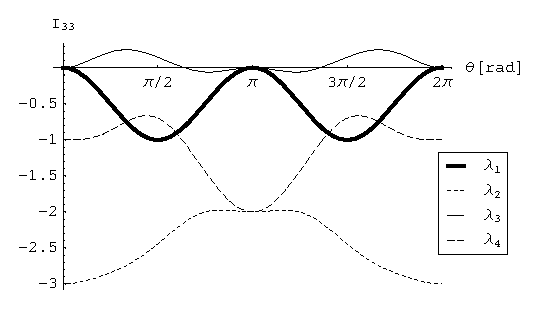
\includegraphics[width=120mm]{2004-qbounds-f11}
\end{itemize}
 }


\frame{
\centerline{\Large Thank you for your attention!}
 }

\end{document}
